\documentclass[tikz]{standalone}
\usepackage{tikz}
\usepackage{siunitx}
\DeclareSIUnit\degF{\text{°}F}

\definecolor{codeblue}{RGB}{69, 161, 248}
\definecolor{codegray}{RGB}{40, 40, 40}
\usetikzlibrary{shapes,arrows}
\tikzstyle{decision} = [diamond, draw, fill=codegray, text=white,
    text width=4.5em, text badly centered, node distance=3cm, inner sep=0pt]
\tikzstyle{block} = [rectangle, draw, fill=codeblue,  text=white,
    text width=5em, text centered, rounded corners, minimum height=4em]
\tikzstyle{line} = [draw, -latex']


\begin{document}
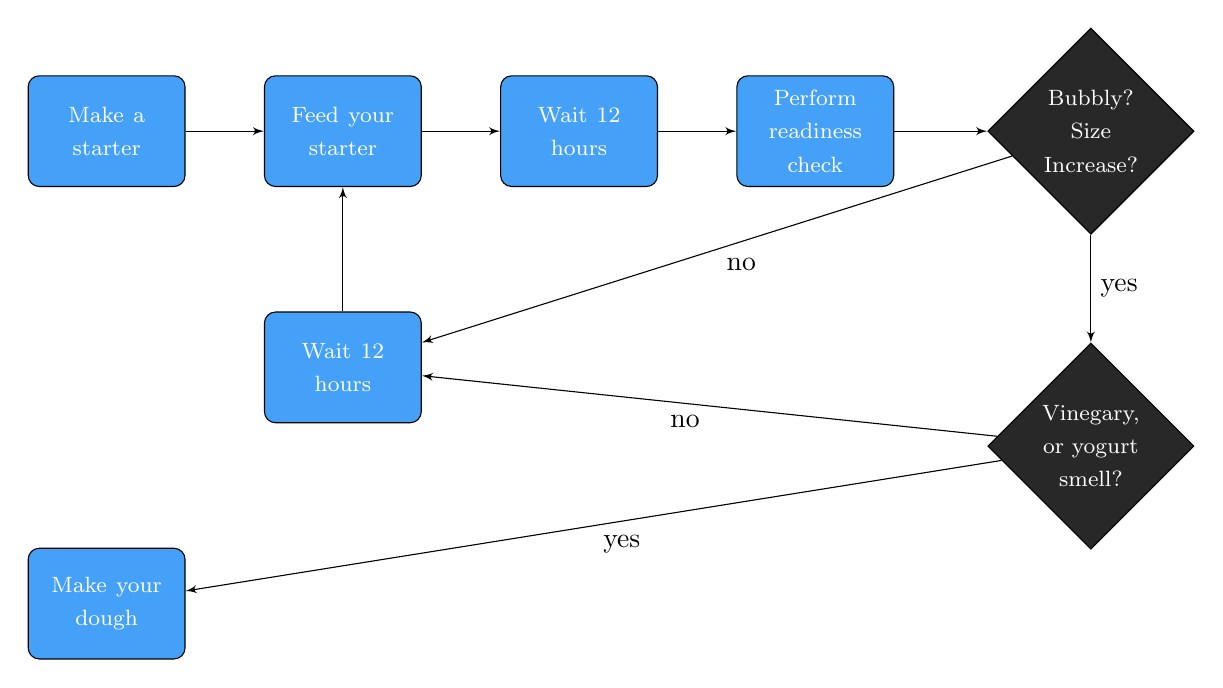
\begin{tikzpicture}[node distance = 3cm, auto]
  \node [block] (init) {\footnotesize Make a starter};
  \node [block, right of=init, node distance=3cm] (feed) {\footnotesize Feed your starter};
  \path [line] (init) -- (feed);
  \node [block, right of=feed, node distance=3cm] (wait_12_after_feed) {\footnotesize Wait 12 hours};
  \path [line] (feed) -- (wait_12_after_feed);
  \node [block, right of=wait_12_after_feed, node distance=3cm] (ready_question) {\footnotesize Perform readiness check};
  \path [line] (wait_12_after_feed) -- (ready_question);
  \node [block, below of=feed, node distance=3cm] (wait_12) {\footnotesize Wait 12 hours};
  \path [line] (wait_12) -- (feed);
  \node [decision, right of=ready_question, node distance=3.5cm] (is_bubbly) {\footnotesize Bubbly? Size Increase?};
  \path [line] (ready_question) -- (is_bubbly);
  \path [line] (is_bubbly) -- node{no} (wait_12);
  \node [decision, below of=is_bubbly, node distance=4.0cm] (check_smell) {\footnotesize Vinegary, or yogurt smell?};
  \path [line] (is_bubbly) -- node{yes} (check_smell);
  \node [block, below of=init, node distance=6cm] (make_dough) {\footnotesize Make your dough};
  \path [line] (check_smell) -- node{yes} (make_dough);
  \path [line] (check_smell) -- node{no} (wait_12);
\end{tikzpicture}
\end{document}
